\documentclass[a4paper,11pt,aps,superscriptaddress]{revtex4}
%%%%%%%%%%%%%%%%%%%%%%%%%%%%%%%%%%%%%%%%%%%%%%%%%%%%%%%%%%%%%%%%%%%%%%%%%%%%%%%%%%%%%%%%%%%%%%%%%%%%%%%%%%%%%%%%%%%%%%%%%%%%%%%%%%%%%%%%%%%%%%%%%%%%%%%%%%%%%%%%%%%%%%%%%%%%%%%%%%%%%%%%%%%%%%%%%%%%%%%%%%%%%%%%%%%%%%%%%%%%%%%%%%%%%%%%%%%%%%%%%%%%%%%%%%%%
%\usepackage[margin=1in]{geometry}
%\usepackage{fullpage}

\usepackage{latexsym}
\usepackage{amsthm}
\usepackage{amssymb}
\usepackage{amsmath}

%\usepackage[all,knot,poly]{xy}
\usepackage[all]{xy}
\usepackage{graphicx}
%\usepackage{epsfig}
\usepackage{subfigure}

%\usepackage{hyperref}

\usepackage{dcolumn} % Align table columns on decimal point
\usepackage{bm} % bold math
\usepackage{color}

%\usepackage{cmbright}
\SelectTips{eu}{11}

\usepackage[a4paper,pagebackref=true,colorlinks=true,
linkcolor=blue,citecolor=blue,
pdfauthor={ },
pdftitle={ },
pdfsubject={ },
pdfkeywords={ }]{hyperref}



\newtheorem*{theorem}{Theorem}
\newtheorem*{proposition}{Proposition}
\newtheorem*{lemma}{Lemma}



\begin{document}

\title{Supplementary Material:\\ ``Maximally Accessible Purity  in Coherently Controlled Open Quantum Systems: Application to Quantum State Engineering"}
\maketitle

\author{Jun Li, Dawei Lu, Zhihuang Luo, Raymond Laflamme, Xinhua Peng, Jiangfeng Du}



\section{Proof of the first proposition}
The proof is based on the majorization method. See \cite{HJ} for a brief introduction of the concept of majorization. We will need the following lemma.
\begin{lemma}
Let $\rho$ be a $2^n$-dimensional density matrix. Then for any unitary $U \in SU(2^n)$, the diagonal part of $U \rho U^{\dag}$ can be written as a convex combination of all permutations of the diagonal part of $\rho$. That is, let $\mathcal{P}_{2^n}$ denote the collection of $2^n!$ permutation operations on diagonal elements, then
\begin{equation}
d(U\rho {U^\dag }) = \sum\limits_{k = 1}^{{2^n!}} {{\mu _k}{P_k}d(\rho )} ,
\end{equation}
where ${P_k} \in {\mathcal{P}_{{2^n}}}$, $\mu_k \ge 0$ and $\sum\nolimits_{k = 1}^{{2^n!}} {{\mu _k}}  = 1$.
\end{lemma}

\begin{proof}
See \textbf{Theorem 4.3.45} (\textbf{Schur}) at p.249 and \textbf{Theorem 4.3.49} at p253 in \cite{HJ}.
\end{proof}



Back to our proposition. The projected dynamics in the representative region goes
\begin{equation}
\label{Projection}
\bm{\dot x} = - {\left[ {{\mathbf{U}^T}\mathbf{R}\mathbf{U}} \right]_\mathbf{p}}(\bm{x} - {\mathbf{U}^T}{\bm{x}_{eq}}).
\end{equation}
Then there is
\begin{equation}
\dot p |_\mathbf{U} =  - 2{(\mathbf{U}{\bm{x}})^T}\mathbf{R}(\mathbf{U}{\bm{x}} - {\bm{x}_{eq}}).
\end{equation}
We state the proposition again
\begin{proposition}
Let $\mathcal{P}_{2^n}$ denote the collection of $2^n!$ permutation operations on diagonal elements. Let $\mathcal{Q}_{2^n}$ be the corresponding set of $\mathcal{P}_{2^n}$ in the vector of coherence representation. Suppose that the relaxation matrix satisfies $\mathbf{R} =  \mathbf{R_p} \oplus \mathbf{R_c}$ and ${\lambda _{\max }}({\mathbf{R_p}}) \le {\lambda _{\min }}({\mathbf{R_c}})$, then there exists an element $\mathbf{Q}$ of $\mathcal{Q}_{2^n}$ such that for any possible unitary $\mathbf{U}$ there is
\begin{equation}
\dot p |_\mathbf{U} \le  - 2{(\mathbf{Q}{\bm{x}})^T}\mathbf{R}(\mathbf{Q}{\bm{x}} - {\bm{x}_{eq}}).
\end{equation}
\end{proposition}


\begin{proof}
Let $\mathbf{U}{\bm{x}} = {\bm{r}_\mathbf{p}} + {\bm{r}_\mathbf{c}}$. By lemma, we have ${\bm{r}_\mathbf{p}} = \sum\limits_{k = 1}^{2^n!} {{\mu_k \mathbf{Q}_k}{\bm{x}}} $. Then
\begin{align}
\dot p |_\mathbf{U} =  & - 2\sum\limits_{k = 1}^{2^n!} {\sum\limits_{j = 1}^{2^n!} {{{\left( {{\mu _k}{\mathbf{Q}_k}{\bm{x}}} \right)}^T}\mathbf{R}\left( {{\mu _j}{\mathbf{Q}_j}\bm{x} - {\bm{x}_{eq}}} \right)} }  - 2\bm{r}_\mathbf{c}^T \mathbf{R} {\bm{r}_\mathbf{c}} \nonumber \\
\le & - 2\sum\limits_{k = 1}^{2^n!} {\sum\limits_{j = 1}^{2^n!} {{{\left( {{\mu _k}{\mathbf{Q}_k}{\bm{x}}} \right)}^T}{\mathbf{R}_\mathbf{p}}\left( {{\mu _j}{\mathbf{Q}_j}{\bm{x}} - {\bm{x}_{eq}}} \right)} }  - 2{\lambda _{\min }}({\mathbf{R}_\mathbf{c}})\bm{r}_\mathbf{c}^T {\bm{r}_\mathbf{c}} \nonumber \\
\le &  - 2\sum\limits_{k = 1}^{2^n!} {\sum\limits_{j = 1}^{2^n!} {{{\left( {{\mu _k}{\mathbf{Q}_k}{\bm{x}}} \right)}^T}{\mathbf{R}_\mathbf{p}}\left( {{\mu _j}{\mathbf{Q}_j}{\bm{x}} - {\bm{x}_{eq}}} \right)} }  - 2{\lambda _{\max }}({\mathbf{R}_\mathbf{p}})\bm{r}_\mathbf{c}^T {\bm{r}_\mathbf{c}} \nonumber \\
\le &  - 2\sum\limits_{k = 1}^{2^n!} {\sum\limits_{j = 1}^{2^n!} {{{\left( {{\mu _k}{\mathbf{Q}_k}{\bm{x}}} \right)}^T}{\mathbf{R}_\mathbf{p}}\left( {{\mu _j}{\mathbf{Q}_j}{\bm{x}} - {\bm{x}_{eq}}} \right)} }   \nonumber \\
& - 2{\lambda _{\max }}({\mathbf{R}_\mathbf{p}})\left[ {\bm{x}^T {\bm{x}} - {{\left( {\sum\limits_{k = 1}^{2^n!} {{\mu _k}{\mathbf{Q}_k}{\bm{x}}} } \right)}^T}\left( {\sum\limits_{j = 1}^{2^n!} {{\mu _j}{\mathbf{Q}_j}{\bm{x}}} } \right)} \right] \nonumber  \\
= &   - 2\sum\limits_{k = 1}^{{2^n}!} {\sum\limits_{j = 1}^{{2^n}!} {{\mu _k}{\mu _j}{\bm{x}^T} \left( {\mathbf{Q}_k^T{\mathbf{R}_\mathbf{p}}{\mathbf{Q}_j} + {\lambda _{\max }}({\mathbf{R}_\mathbf{p}}) - {\lambda _{\max }}({\mathbf{R}_\mathbf{p}})\mathbf{Q}_k^T{\mathbf{Q}_j}} \right) \bm{x}} }  \nonumber \\
& + 2\sum\limits_{k = 1}^{{2^n}!} {{\mu _k}{\bm{x}^T}\mathbf{Q}_k^T{\mathbf{R}_\mathbf{p}}{\bm{x}_{eq}}}.
\label{1}
\end{align}
Now we need an inequality
\[{({\mathbf{Q}_k} - {\mathbf{Q}_j})^T}({\mathbf{R}_\mathbf{p}} - {\lambda _{\max }}({\mathbf{R}_\mathbf{p}}))({\mathbf{Q}_k} - {\mathbf{Q}_j}) \le 0,\]
the correctness of which is easy to check. Expand the inequality we have
\begin{align}
&  - (\mathbf{Q}_k^T{\mathbf{R}_\mathbf{p}}{\mathbf{Q}_j} + \mathbf{Q}_j^T{\mathbf{R}_\mathbf{p}}{\mathbf{Q}_k} + {\lambda _{\max }}({\mathbf{R}_\mathbf{p}})\mathbf{I} + {\lambda _{\max }}({\mathbf{R}_\mathbf{p}})\mathbf{I} - {\lambda _{\max }}({\mathbf{R}_\mathbf{p}})\mathbf{Q}_k^T{\mathbf{Q}_j} - {\lambda _{\max }} ({\mathbf{R}_\mathbf{p}}) \mathbf{Q}_j^T{\mathbf{Q}_k}) \nonumber \\
\le & - {\mathbf{Q}_k^T}{\mathbf{R}_\mathbf{p}}{\mathbf{Q}_k} - {\mathbf{Q}_j^T}{\mathbf{R}_\mathbf{p}}{\mathbf{Q}_j}.  \nonumber
\end{align}
Substitute into Eq. (\ref{1}), we get
\begin{align}
\dot p |_\mathbf{U} &  \le    - 2\sum\limits_{k = 1}^{{2^n}!} {\sum\limits_{j = 1}^{{2^n}!} {{\mu _k}{\mu _j}{\bm{x}^T} \left( {{\mathbf{Q}_k^T{\mathbf{R}_\mathbf{p}}{\mathbf{Q}_k} + \mathbf{Q}_j^T{\mathbf{R}_\mathbf{p}}{\mathbf{Q}_j}}} \right) \bm{x}} }   + 2\sum\limits_{k = 1}^{{2^n}!} {{\mu _k}{\bm{x}^T}\mathbf{Q}_k^T{\mathbf{R}_\mathbf{p}}{\bm{x}_{eq}}} \nonumber  \\
& =  - 2 \sum\limits_{k = 1}^{{2^n}!} {{\mu _k}{\bm{x}^T}\mathbf{Q}_k^T{\mathbf{R}_\mathbf{p}}{\mathbf{Q}_k}\bm{x}} + 2\sum\limits_{k = 1}^{{2^n}!} {{\mu _k}{\bm{x}^T}\mathbf{Q}_k^T{\mathbf{R}_\mathbf{p}}{\bm{x}_{eq}}}  \nonumber \\
& = - 2\sum\limits_{k = 1}^{{2^n}!} {{\mu _k}{{\left( {{\mathbf{Q}_k}\bm{x}} \right)}^T}{\mathbf{R}_\mathbf{p}}\left( {({\mathbf{Q}_k}\bm{x}) - {\bm{x}_{eq}}} \right)}.
\end{align}
Note that the last line is a convex combination, the proposition is proved.
\end{proof}


\section{Proof of the second proposition}
We here state the second proposition again
\begin{proposition}
Each element $\mathbf{Q}_k$ ($k=1,...,2^n!$) in $\mathcal{Q}_{2^n}$ is associated with two definite quadratic forms��
\begin{align}
& E_k =  - 2{(\mathbf{Q}_k {\bm{x}})^T} \mathbf{R} (\mathbf{Q}_k {\bm{x}} - {\bm{x}_{eq}}),  \nonumber \\
& F_k = 4 {(\mathbf{Q}_k{\bm{x}} - {\bm{x}_{eq}}/2)^T} \mathbf{R}^2 (\mathbf{Q}_k{\bm{x}} - {\bm{x}_{eq}}).
\end{align}
Because of permutation symmetry, there exists a constant $C$ such that for each $k$, $E_k = C$ is the smallest ellipsoid enclosing $F_k = 0$.
Then in the representative region $\Sigma$,  it is impossible to steer system from $\bm{x}_{eq}$ to any state that locates outside the ellipsoid
\begin{equation}
E: - 2{{\bm{x}}^T} \mathbf{R} ( {\bm{x}} - {\bm{x}_{eq}}) = C,
\end{equation}
through ${\left[ {\tau } - {V}  \right]_m}$ type of control sequences.
\end{proposition}

\begin{proof}
We  show the following points at first: (i) it is direct to check that $E_k$ represents $\dot p |_{\mathbf{Q}_k}$, and $F_k$ represents $\ddot p|_{\mathbf{Q}_k}$ for diagonal free relaxation dynamics; (ii) there always exists a point $\mathbf{Q}^T_k \bm{x}_{eq}$ such that $E_k(\bm{x}) = 0$ and $F_k(\bm{x}) = 0$, therefore $C \le 0$; (iii) under pure relaxation, for any diagonal state $\rho$, if $\dot p (\rho) = C$, then $\ddot p (\rho) \ge 0$. This implies that if the system starts at a diagonal state $\rho (0)$ satisfying $\dot p(\rho (0)) \ge C$, then under pure relaxation, $\dot p(\rho (t)) \ge C$ for all $t$.

Let $\bm{x}_{ss}$ locates outside $E$.  Back to the density matrix representation $\bm{x}_{ss} \to \rho_{ss}$, there is $\dot p(\bm{\rho}_{ss}) < C$. Suppose the steady state is fixed by ${\left[ {V} - {\tau } \right]_m}$, we have $\mathcal{E}_{\tau} \circ \mathcal{E}_V \rho_{ss} =\rho_{ss}$, which means that the coherences produced after $\mathcal{E}_V$ vanishes by $\mathcal{E}_{\tau}$. Since the relaxation process in diagonal subspace is independent from that in coherence subspace, we get $\mathcal{E}_{\tau} \circ \mathcal{E}_D \circ \mathcal{E}_V\rho_{ss} = \rho_{ss} $, where $\mathcal{E}_D$ means projection into the diagonal subspace. Now,
(i) if $\dot p (\mathcal{E}_D \circ \mathcal{E}_V\rho_{ss}) \ge C$, then after pure relaxation $\mathcal{E}_{\tau}$, there remains $\dot p (\mathcal{E}_{\tau} \circ \mathcal{E}_D \circ \mathcal{E}_V\rho_{ss}) \ge C $, which can not be equal to $\rho_{ss}$; (ii) Otherwise if $\dot p (\mathcal{E}_D \circ \mathcal{E}_V\rho_{ss})  \le C$, then $p$ is decreasing. In order that after $\mathcal{E}_{\tau}$ system is of the same purity as $\rho_{ss}$, there must exist $\tau_0 < \tau$ such that $\dot p (\mathcal{E}_{\tau_0} \circ \mathcal{E}_D \circ \mathcal{E}_V\rho_{ss}) = 0$. As $C \le 0$, there should be $\dot p (\mathcal{E}_{\tau} \circ \mathcal{E}_D \circ \mathcal{E}_V\rho_{ss}) \ge C$, and $\rho_{ss}$ can not be retained either.
\end{proof}


\section{Relaxation Matrix Tomography on Chloroform}
The basic liquid NMR relaxation theory can be found in \cite{KM}. In the rotating frame, it is routine to make a secular approximation by which the relaxation matrix would take a kite-like appearance.
The underlying principle is that, the system energy level differences are much larger than the relaxation rates, so in the interaction picture, the cross relaxation parameters between the population subspace and the coherence subspace are added with fast oscillating phases. This effectively decoupled the population subspace relaxation from the coherence subspace relaxation.
Secular approximation dramatically simplified the task of experimentally estimating the relaxation rates.

To be concrete, the relaxation dynamics can be decomposed as a direct sum of subspace dynamics (featured by the order of coherences)
\begin{itemize}
\item{population subspace:
\begin{equation}
\frac{d}{{dt}}\left( {\begin{array}{*{20}{c}}
   {1/4}  \\
   {\left\langle {ZI} \right\rangle }  \\
   {\left\langle {IZ} \right\rangle }  \\
   {\left\langle {ZZ} \right\rangle }  \\
\end{array}} \right) = \left[ {\begin{array}{*{20}{c}}
   0 & 0 & 0 & 0  \\
   { - (4{r_1} + 16{r_4})\varepsilon } & {{r_1}} & {{r_4}} & {{r_5}}  \\
   { - (4{r_4} + 16{r_2})\varepsilon } & {{r_4}} & {{r_2}} & {{r_6}}  \\
   { - (4{r_5} + 16{r_6})\varepsilon } & {{r_5}} & {{r_6}} & {{r_3}}  \\
\end{array}} \right]\left( {\begin{array}{*{20}{c}}
   {1/4}  \\
   {\left\langle {ZI} \right\rangle }  \\
   {\left\langle {IZ} \right\rangle }  \\
   {\left\langle {ZZ} \right\rangle }  \\
\end{array}} \right),
\end{equation}
}
\item{subspace of $^{13}$C one coherences:
\begin{equation}
\frac{d}{{dt}}\left( {\begin{array}{*{20}{c}}
   {\left\langle {XI} \right\rangle }  \\
   {\left\langle {YI} \right\rangle }  \\
   {\left\langle {XZ} \right\rangle }  \\
   {\left\langle {YZ} \right\rangle }  \\
\end{array}} \right) = \left[ {\begin{array}{*{20}{c}}
   r_7 & 0 & r_9 & -\pi J  \\
   0 & r_7 & \pi J & r_9  \\
   r_9 & -\pi J & r_8 & 0  \\
   \pi J & {{r_9}} & 0 & r_8  \\
\end{array}} \right]\left( {\begin{array}{*{20}{c}}
  {\left\langle {XI} \right\rangle }  \\
   {\left\langle {YI} \right\rangle }  \\
   {\left\langle {XZ} \right\rangle }  \\
   {\left\langle {YZ} \right\rangle }  \\
\end{array}} \right),
\end{equation}
}
\item{subspace of H one coherences:
\begin{equation}
\frac{d}{{dt}}\left( {\begin{array}{*{20}{c}}
  {\left\langle {IX} \right\rangle }  \\
   {\left\langle {IY} \right\rangle }  \\
   {\left\langle {ZX} \right\rangle }  \\
   {\left\langle {ZY} \right\rangle }  \\
\end{array}} \right) = \left[ {\begin{array}{*{20}{c}}
   r_{10} & 0 & r_{12} & -\pi J  \\
   0 & r_{10} & \pi J & r_{12}  \\
   r_{12} & -\pi J & r_{11} & 0  \\
   \pi J & {{r_{12}}} & 0 & r_{11}  \\
\end{array}} \right]\left( {\begin{array}{*{20}{c}}
  {\left\langle {IX} \right\rangle }  \\
   {\left\langle {IY} \right\rangle }  \\
   {\left\langle {ZX} \right\rangle }  \\
   {\left\langle {ZY} \right\rangle }  \\
\end{array}} \right),
\end{equation}
}
\item{:
\begin{equation}
\frac{d}{{dt}}\left( {\begin{array}{*{20}{c}}
   {\left\langle {XY} \right\rangle }  \\
   {\left\langle {YX} \right\rangle }  \\
   {\left\langle {XX} \right\rangle }  \\
   {\left\langle {YY} \right\rangle }  \\
\end{array}} \right) = \left[ {\begin{array}{*{20}{c}}
  r_{13} & -r_{14} & 0 & 0  \\
   -r_{14} & r_{13} & 0 & 0  \\
   0 & 0 & r_{13} & r_{14}  \\
   0 & 0 & r_{14} & r_{13}  \\
\end{array}} \right]\left( {\begin{array}{*{20}{c}}
   {\left\langle {XY} \right\rangle }  \\
   {\left\langle {YX} \right\rangle }  \\
   {\left\langle {XX} \right\rangle }  \\
   {\left\langle {YY} \right\rangle }  \\
\end{array}} \right),
\end{equation}
}
\end{itemize}
where $\left\{r_k \right\}_{k=1,...,14}$ are relaxation rates including auto-relaxation rates and cross-relaxation rates. To estimate the relaxation rates, we first sample the system evolution trajectory (starting from a known initial state $\rho (0)$), then find values of the relaxation rates so that the simulated dynamics can match the observed trajectory. The fitting results are listed below (we have set $\epsilon = 1$)
\begin{itemize}
\item{$\left\{ r_1, r_2, r_3, r_4, r_5, r_6 \right \} \approx \left\{ 0.0532, 0.0918, 0.0798, 0.0212, 0.0000, 0.0022 \right \}$
\begin{figure}[h]
\centering
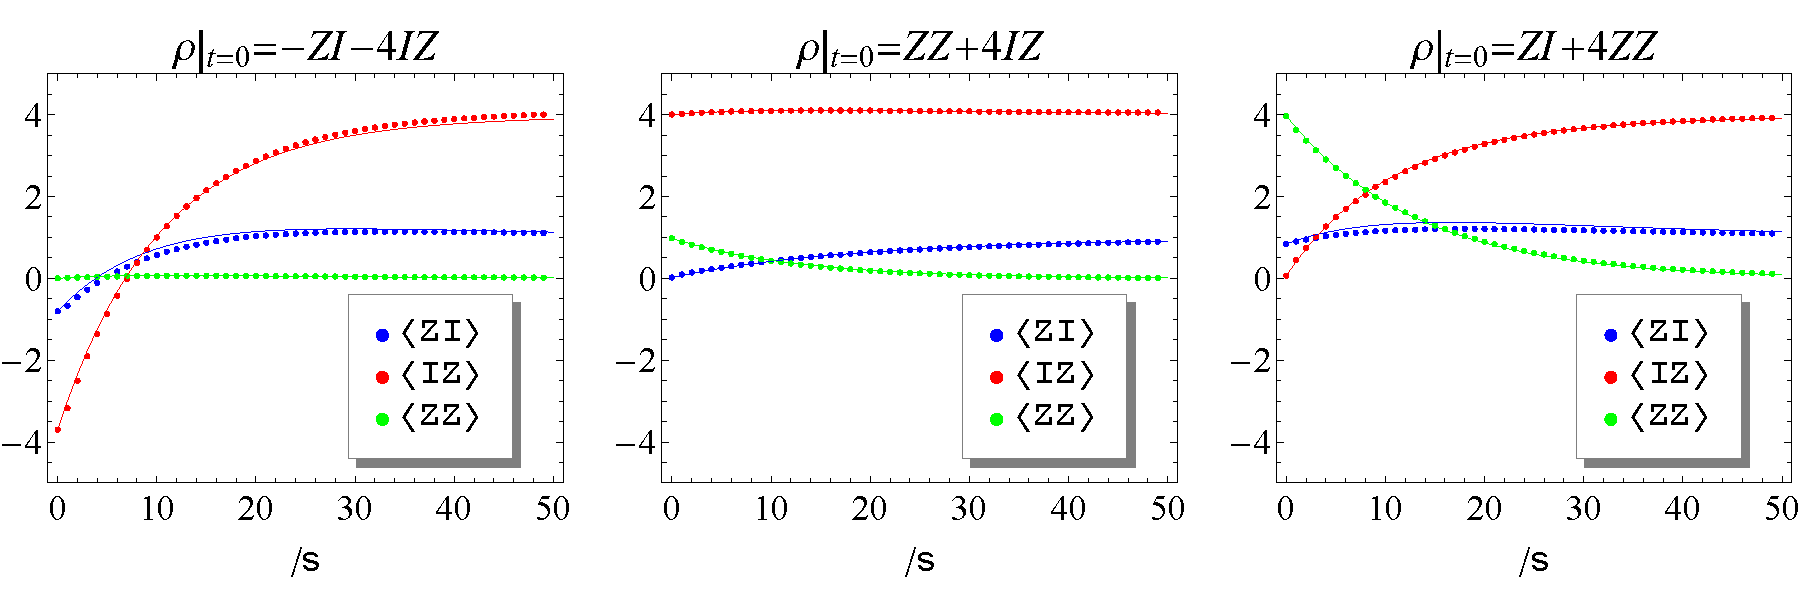
\includegraphics[width=0.9\linewidth]{Population}
\end{figure}
}
\end{itemize}
\newpage
\begin{itemize}
\item{$\left\{ r_7, r_8, r_9 \right \} \approx \left\{ 3.495, 6.536, 0.0100 \right \}$
\begin{figure}[h]
\centering
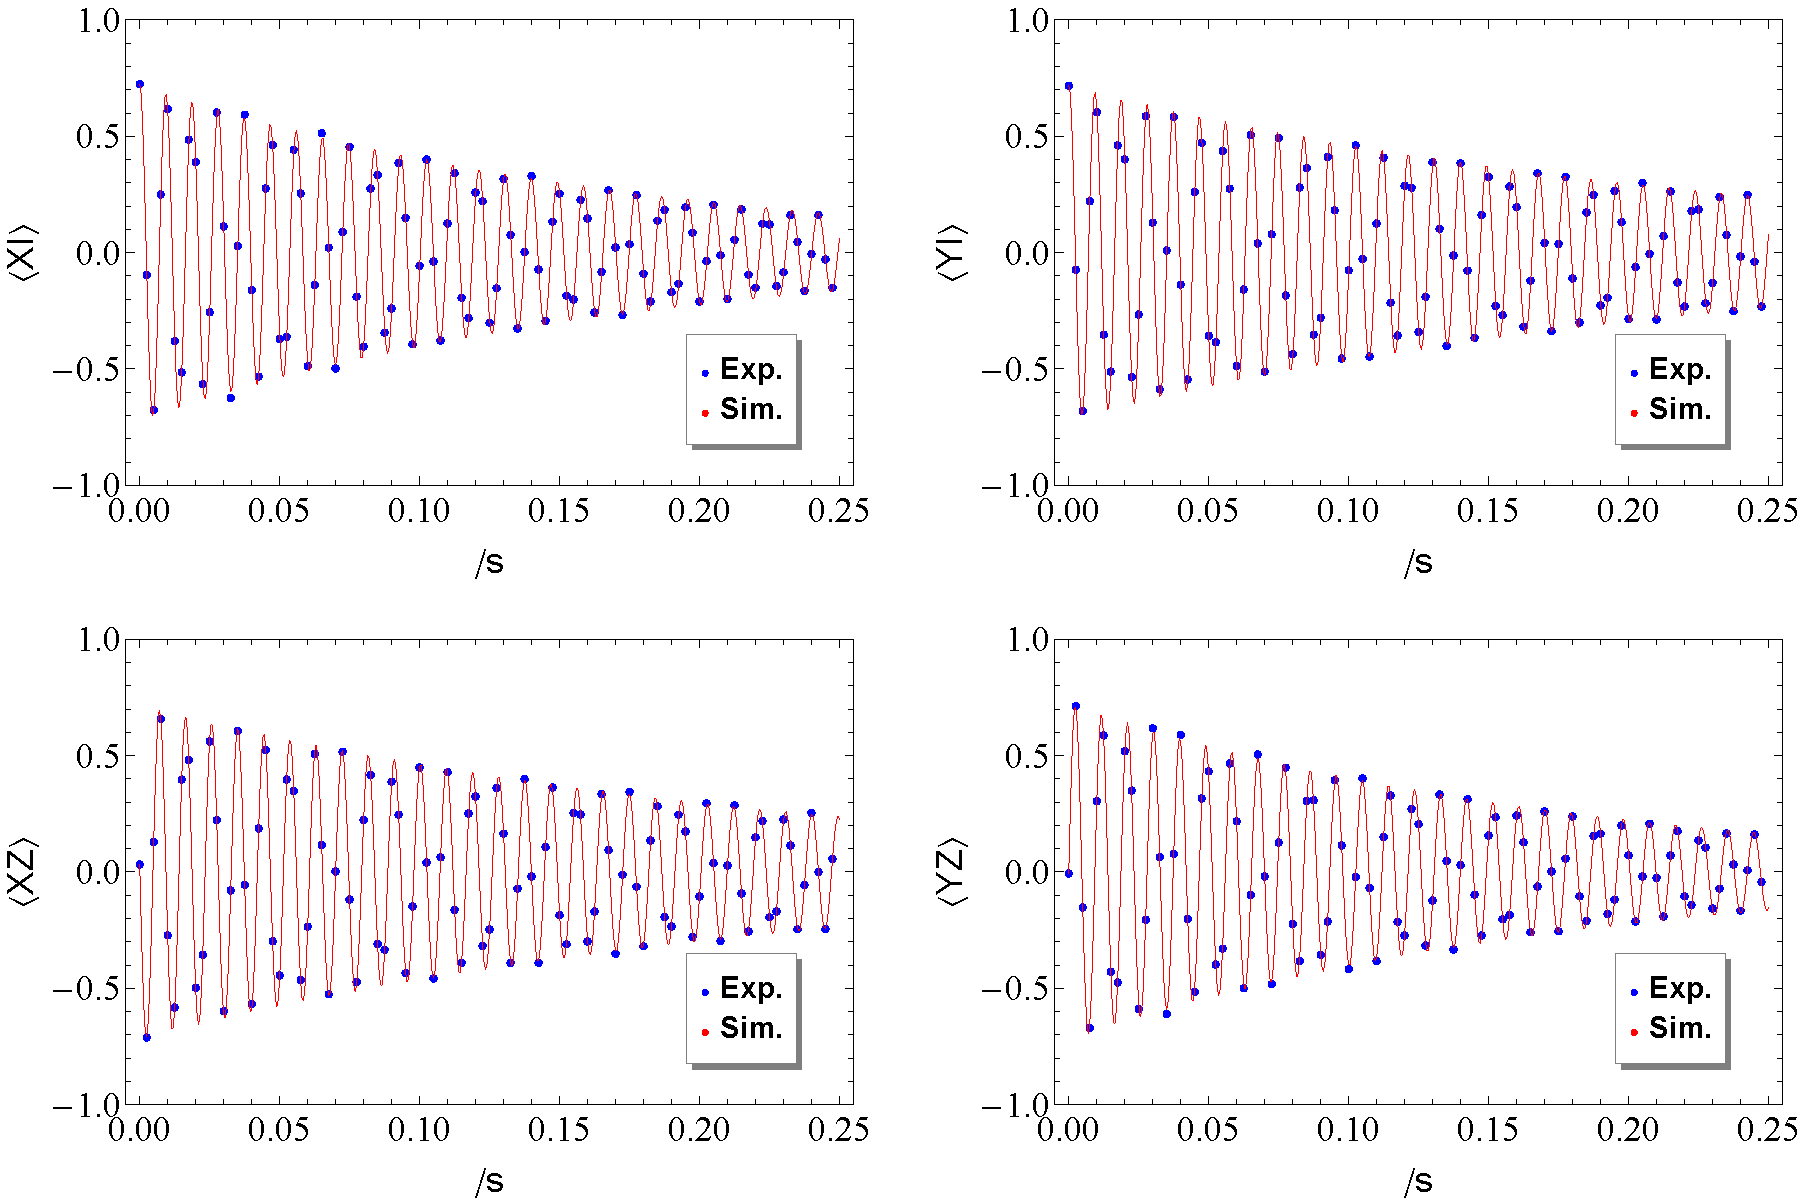
\includegraphics[width=0.8\linewidth]{CCoherence}
\end{figure}
}
\end{itemize}
\begin{itemize}
\item{$\left\{ r_{10}, r_{11}, r_{12} \right \} \approx \left\{ 2.955, 6.118, 0.030 \right \}$
\begin{figure}[h]
\centering
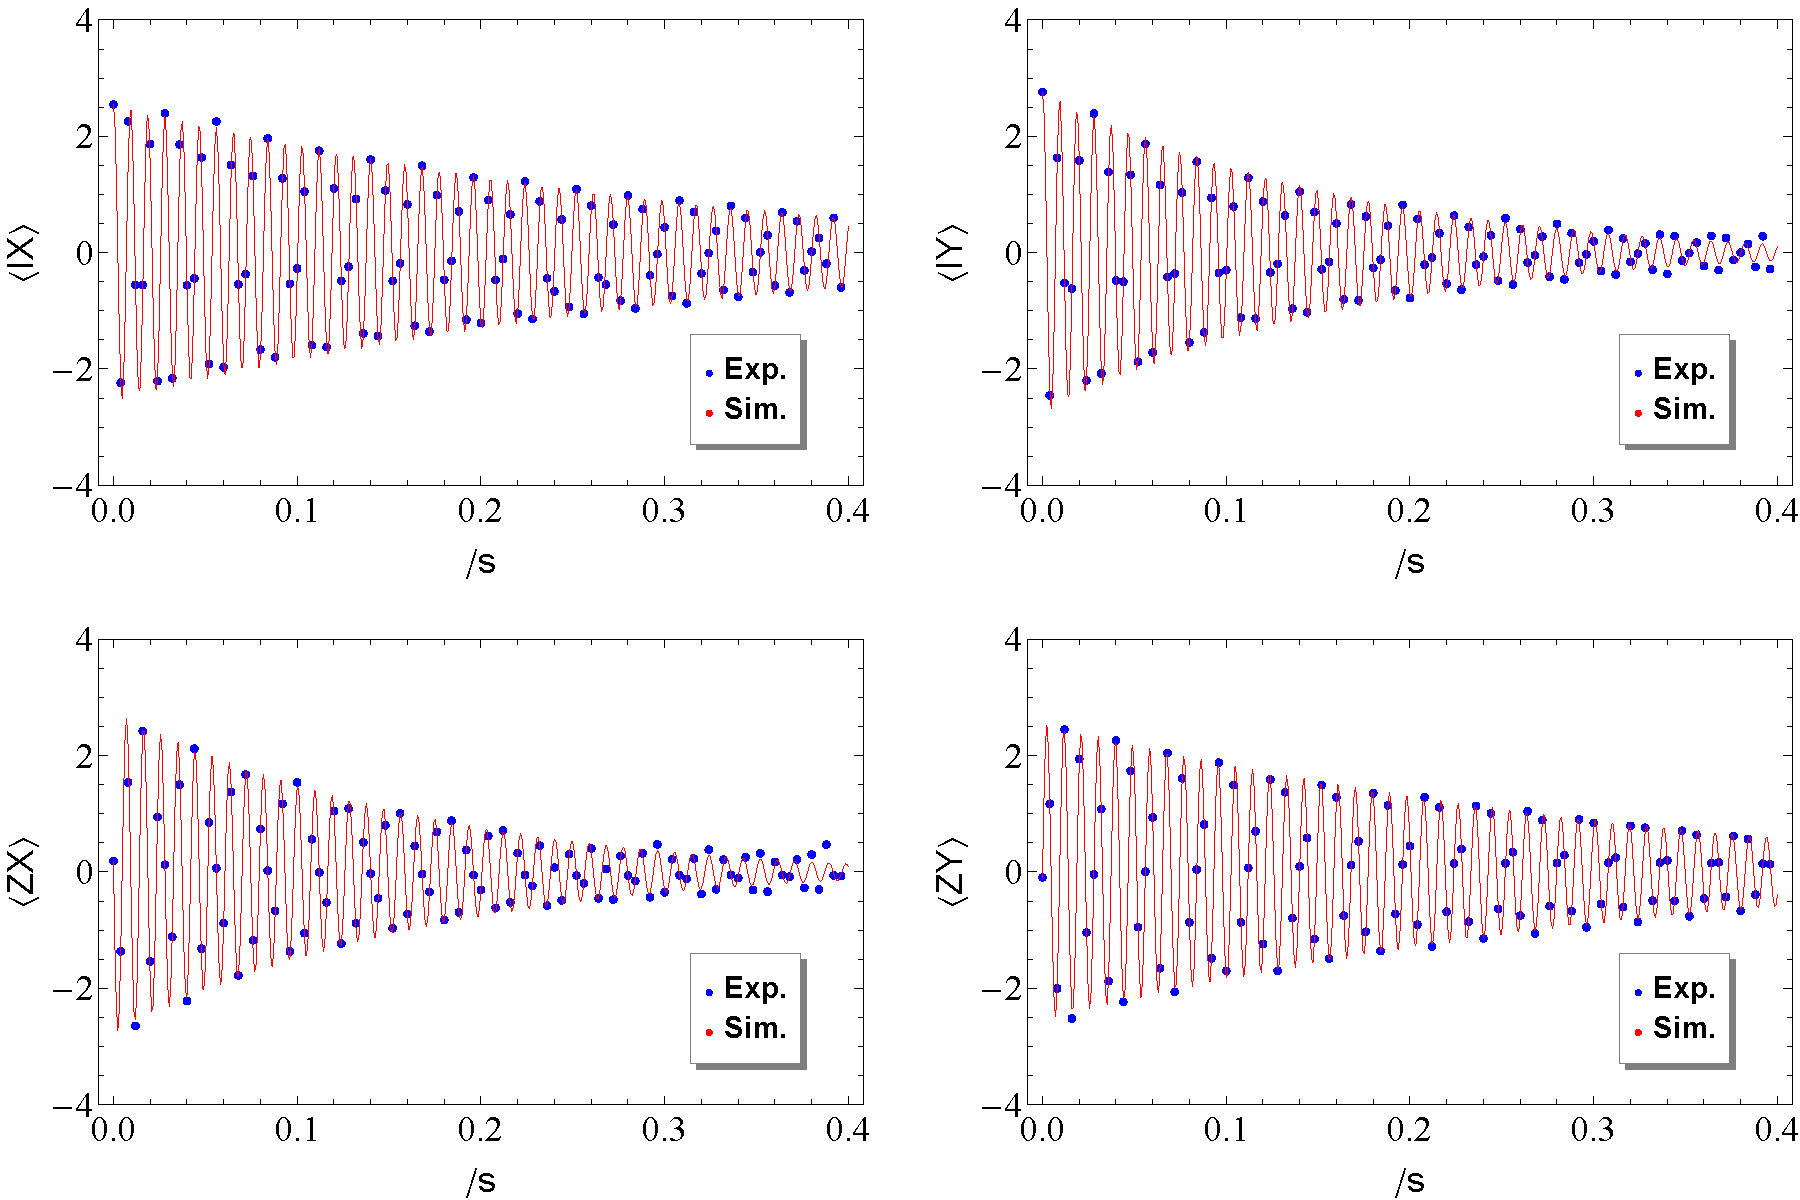
\includegraphics[width=0.8\linewidth]{HCoherence}
\end{figure}
}
\end{itemize}
\begin{itemize}
\item{$\left\{ r_{13}, r_{14} \right \} \approx \left\{ 9.523, 0.008 \right \}$
\begin{figure}[h]
\centering
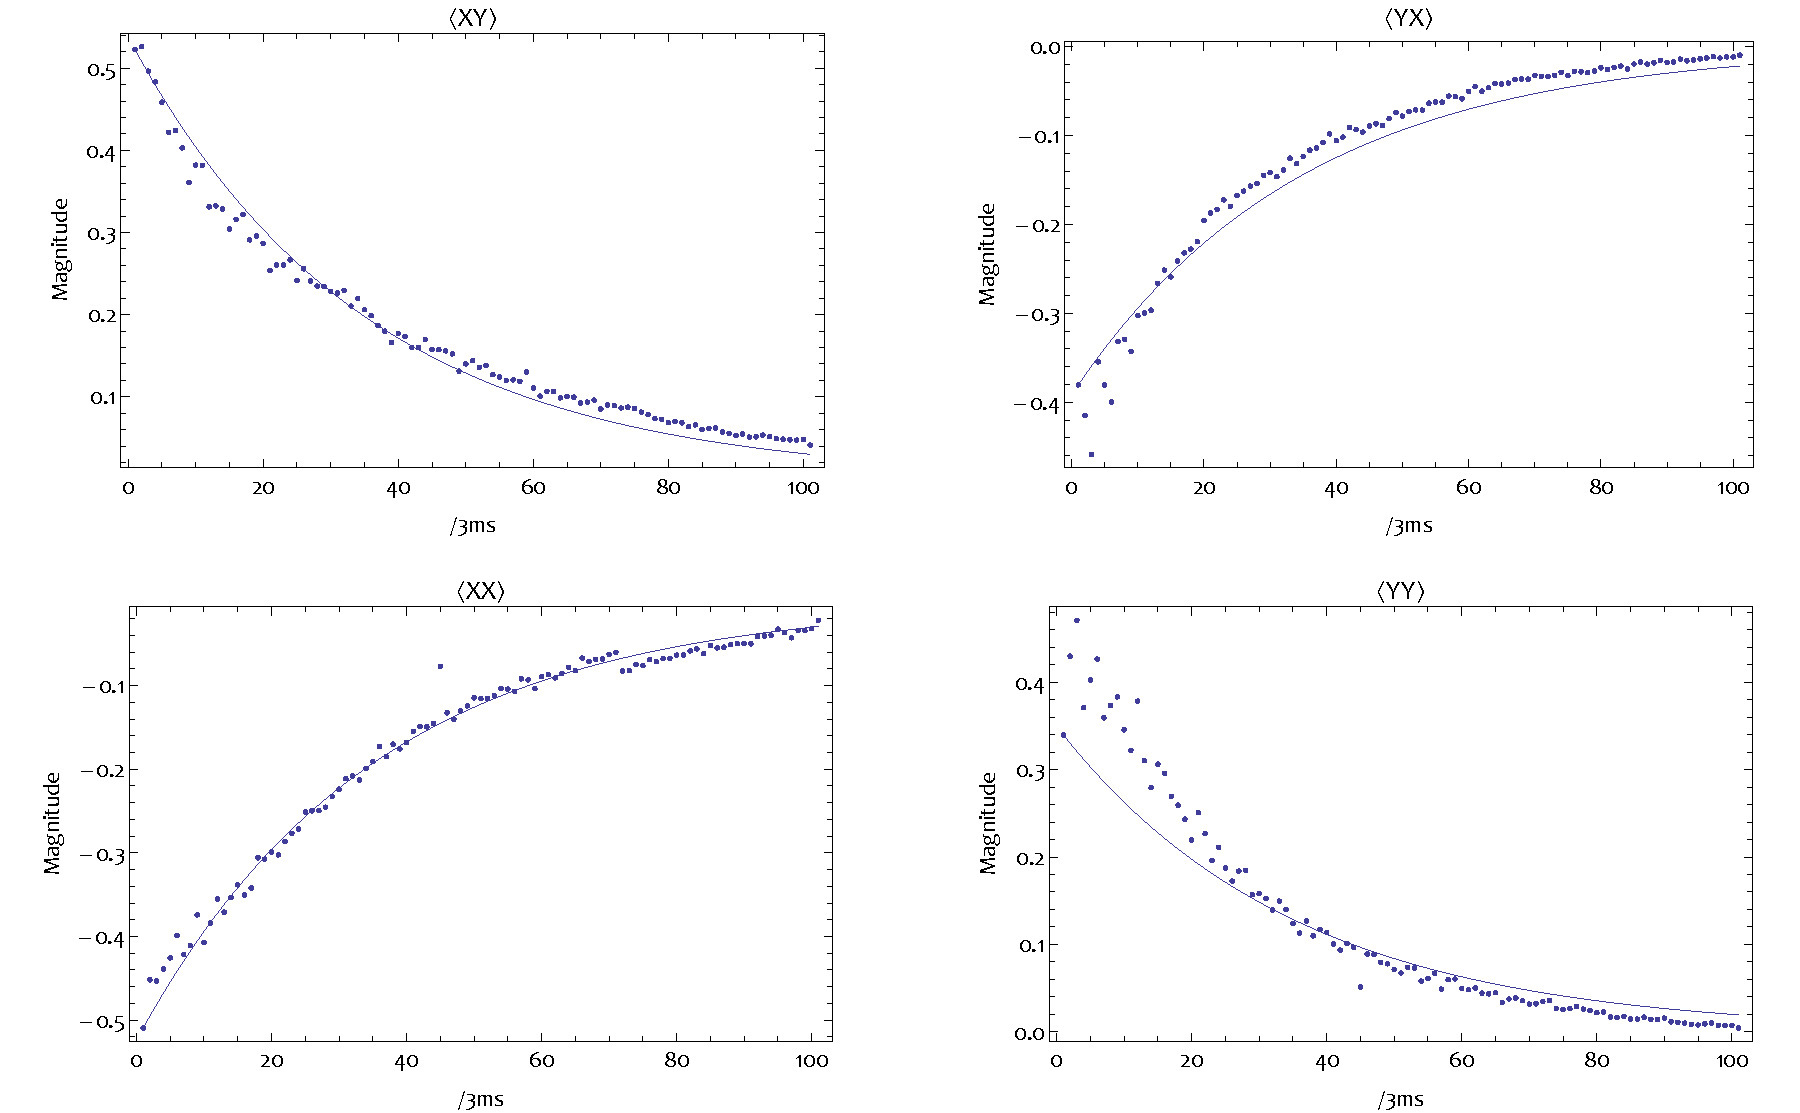
\includegraphics[width=0.75\linewidth]{2Coherence}
\end{figure}
}
\end{itemize}



\newpage

\section{Robustness of Periodic Control Method for PPS Preparation}
The simulating plot shows the relative error of the prepared PPS due to imperfections of control fields present in the $^{13}$C channel ($\delta_{\text{C}} = \left| {B_{real}^{\text{C}} - B_{ideal}^{\text{C}}} \right|{\rm{/}}\left| {B_{ideal}^{\text{C}}} \right|$) and $^1$H channel ($\delta_{\text{H}} = \left| {B_{real}^{\text{H}} - B_{ideal}^{\text{H}}} \right|{\rm{/}}\left| {B_{ideal}^{\text{H}}} \right|$). The relative error is characterized by
\begin{equation}
\delta = \left\| {{\rho _{real}} - {\rho _{pps}}} \right\|/\left\| {{\rho _{pps}}} \right\|.
\end{equation}
It can be easily seen that the periodic control method is quite robust to the control imperfections.
\begin{figure}[h]
  \begin{minipage}[c]{0.6\textwidth}
    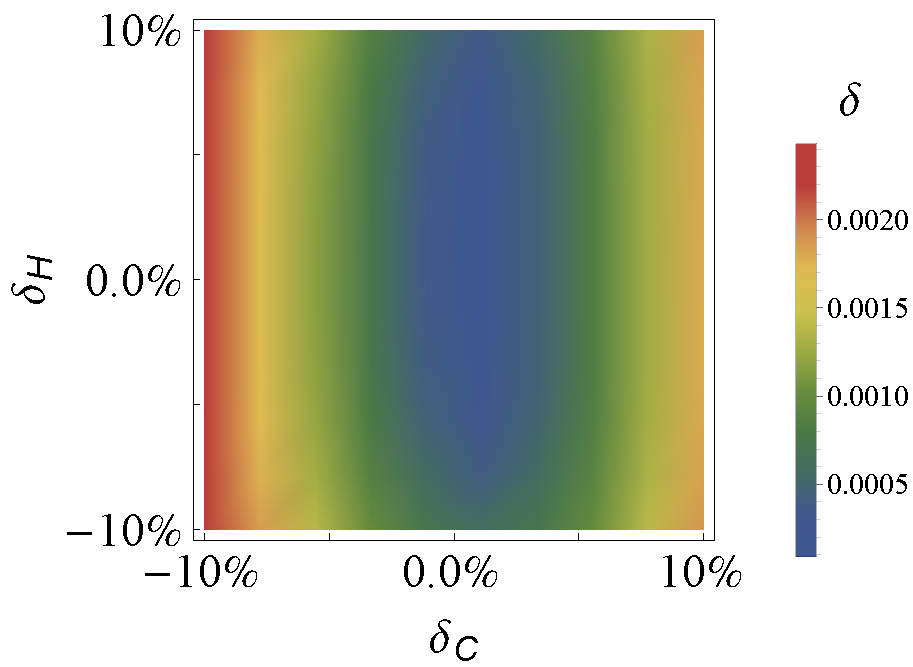
\includegraphics [width=0.8\textwidth]{Robustness}
  \end{minipage}\hfill
  \begin{minipage}[c]{0.4\textwidth}
    \caption{Simulation result: relative error of the prepared PPS due to imperfections of control fields present in the $^{13}$C channel and $^1 $H channel.}
    \label{Robustness}
  \end{minipage}
\end{figure}

\begin{thebibliography}{28}
\bibitem{HJ} R. A. Horn and C. R. Johnson, \emph{Matrix Analysis} (Cambridge University Press, Cambridge, England, 2013).

\bibitem{KM} J. Kowalewski and L. M{\"{a}}ler, \emph{Nuclear Spin Relaxation in Liquids: Theory, Experiments, and Applications} (Taylor \& Francis, New York, 2006).

\end{thebibliography}

\end{document}
